
   \frame{
  \frametitle {Our first simple Docker image}
 To create our image we will perform the following tasks:\vspace{0.4cm}
 \begin{itemize}
 \item Create an own docker public repository;\vspace{0.2cm}
 \item Download a  base image from the Docker Hub;\vspace{0.2cm}		
 \item Updating the download images and upload it on our own repository;\vspace{0.2cm}\color{grey}	
 \item Create and embed  simple BASH and R  scripts on our image;\vspace{0.2cm}	
 \item Execute the new created image.
 \end{itemize}
}  
  
  
        \frame{
\frametitle{Updating the download images and upload it} 
Before updating the downloaded image we have to rename it;\\ \vspace{0.3cm}
\emph{\color{PineGreen} docker tag  $\langle \it{source\_image} \rangle$ $\langle \it{target\_image} \rangle$} can be used to create  a tag $\color{NavyBlue}\langle \it{target\_image} \rangle$ that refers to $\color{NavyBlue}\langle \it{source\_image} \rangle$.
  \vspace{0.2cm}
          	\begin{center}
  			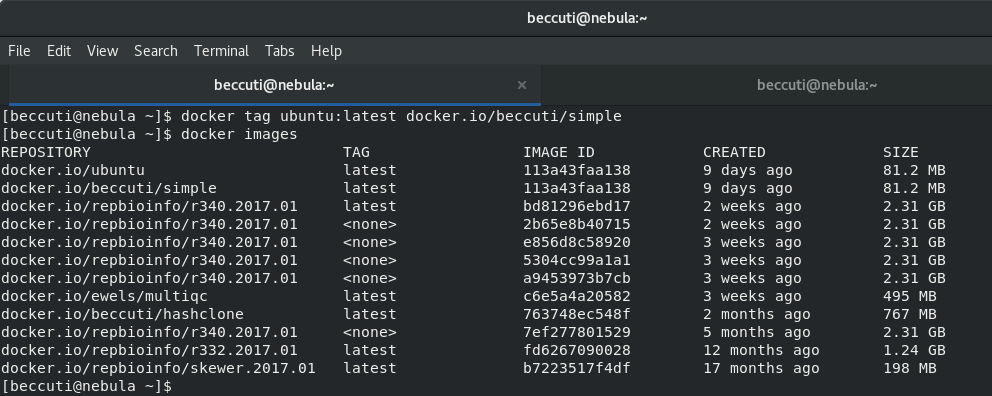
\includegraphics[width=1.0\columnwidth]{./Figure/tag}
  		\end{center}
} 
  	
  	
 	     \frame{
\frametitle{Building a Docker Image} 
  
 \emph{\color{PineGreen} docker run -it $\langle \it{target\_image} \rangle$ /bin/bash} can be used to run a specific docker image interactively.
     	\begin{center}
  			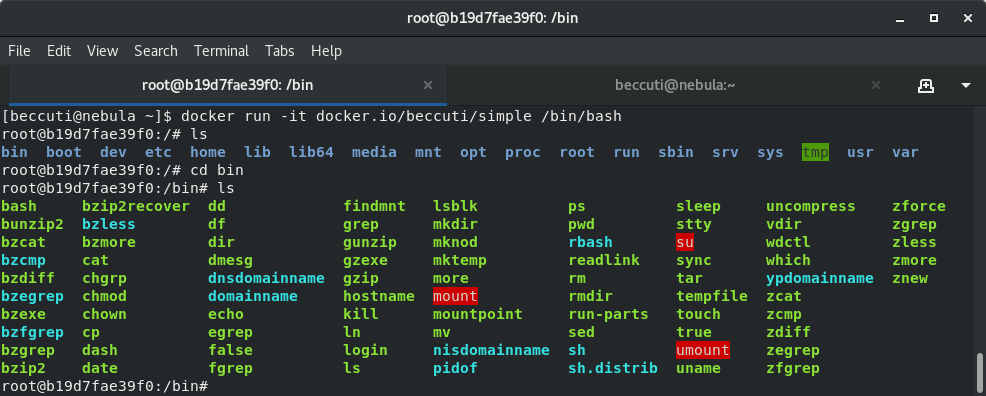
\includegraphics[width=1.00\columnwidth]{./Figure/run}
  		\end{center}  
  
 }  	
  	
\frame{
\frametitle{Building a Docker Images} 
  
Commands can be executed on a container as a remote machine.   \vspace{0.2cm}
     	\begin{center}
  			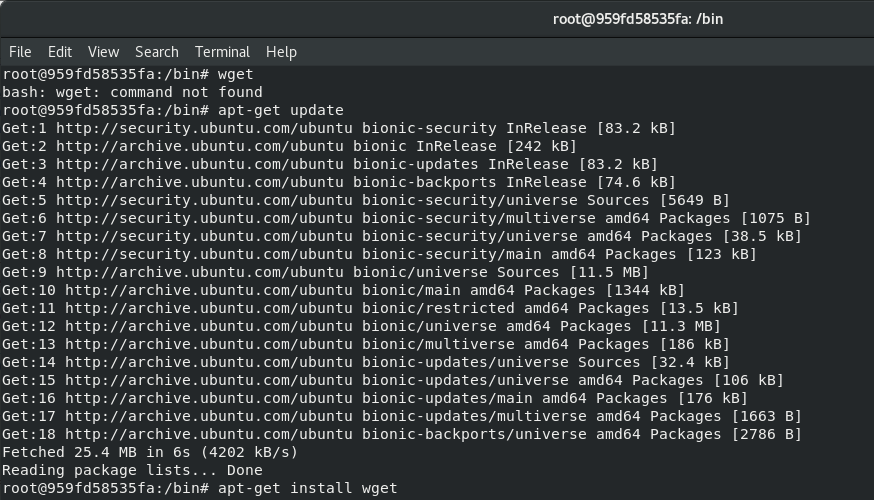
\includegraphics[width=1.00\columnwidth]{./Figure/run2}
  		\end{center}  
  
 }
 
 
    	     \frame{
\frametitle{Building a Docker Image} 
 
 \emph{\color{PineGreen} docker ps -a} can be used  to list the running and executed containers.\vspace{0.2cm}
     	\begin{center}
  			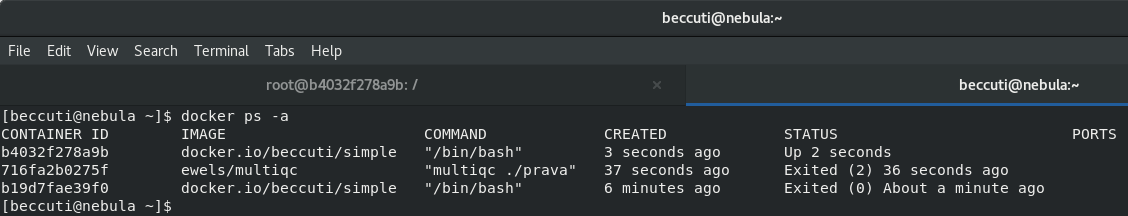
\includegraphics[width=1.01\columnwidth]{./Figure/ps}
  		\end{center}  
  
 }
 
 
  
    	     \frame{
\frametitle{Building a Docker Image} 
 
 \emph{\color{PineGreen} docker ps  -f $\langle \it{filter\_cond} \rangle$} lists only the containers satisfying filter condition.
%     	\begin{center}
 % 			\includegraphics[width=1.00\columnwidth]{./Figure/%ps1}
  %		\end{center}  
       	\begin{center}
  			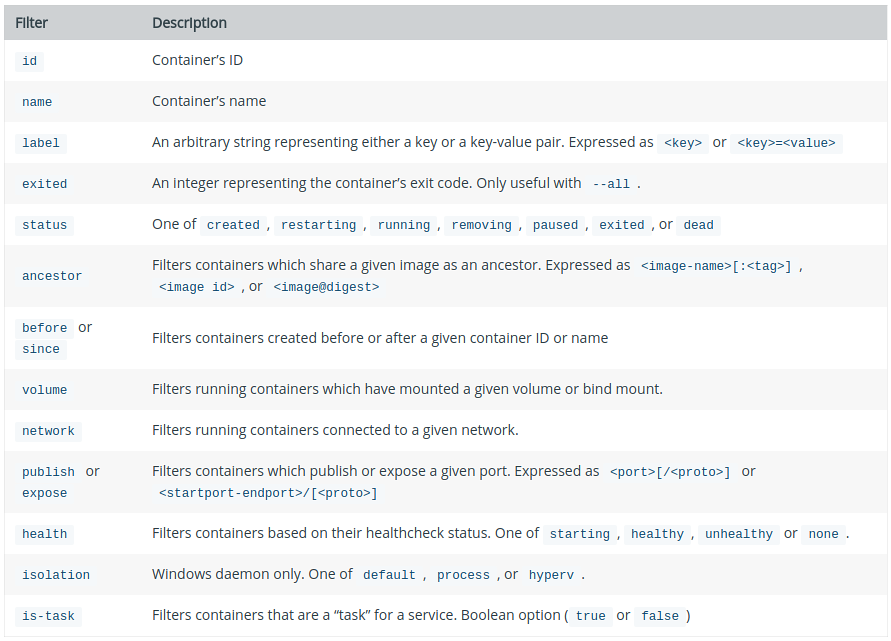
\includegraphics[width=0.90\columnwidth]{./Figure/filter}
  		\end{center}  
 }
     	     \frame{
\frametitle{Building a Docker Image} 
 
 \emph{\color{PineGreen} docker ps -f $\langle \it{filter\_cond} \rangle$} lists only the containers satisfying filter condition.
    	\begin{center}
  			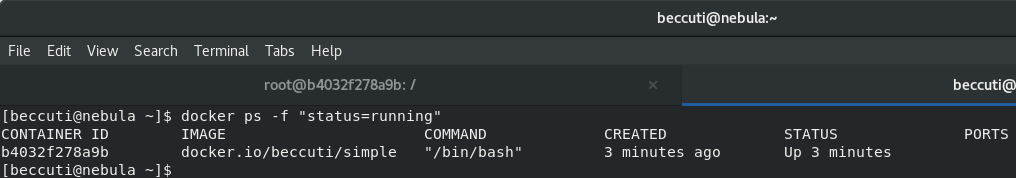
\includegraphics[width=1.00\columnwidth]{./Figure/ps1}
  		\end{center}  
  %     	\begin{center}
  %			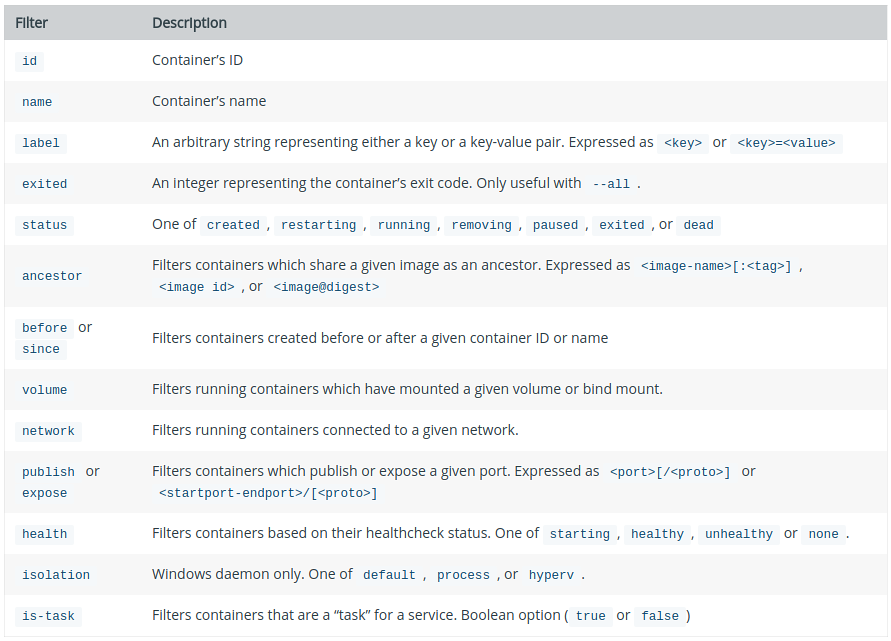
\includegraphics[width=0.90\columnwidth]{./Figure/filter}
  %		\end{center}  
 }
 
 
 
 
 \frame{
\frametitle{Building a Docker Image} 
A commit must be executed to make permanent the image update. \\\vspace{0.1cm}
 \emph{\color{PineGreen} docker commit [ContainerID] [Repository[:Tag]} commits the container image \vspace{0.1cm}
 	     	\begin{center}
  			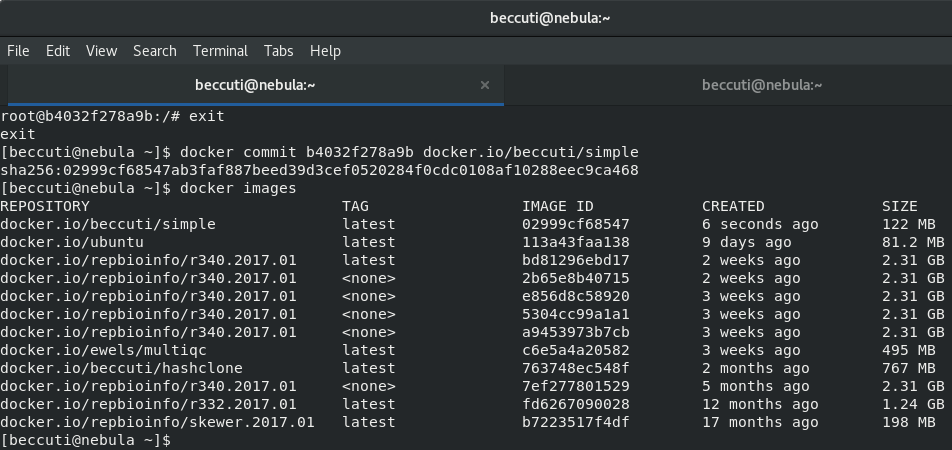
\includegraphics[width=1.0\columnwidth]{./Figure/commit}
  		\end{center}  
 	}
  	
  	
  	
       \frame{
\frametitle{Building a Docker Image} 
  
 \emph{\color{PineGreen} docker push 
 $\langle \it{image} \rangle$} can be used to upload a docker image into  a hub.
     	\begin{center}
  			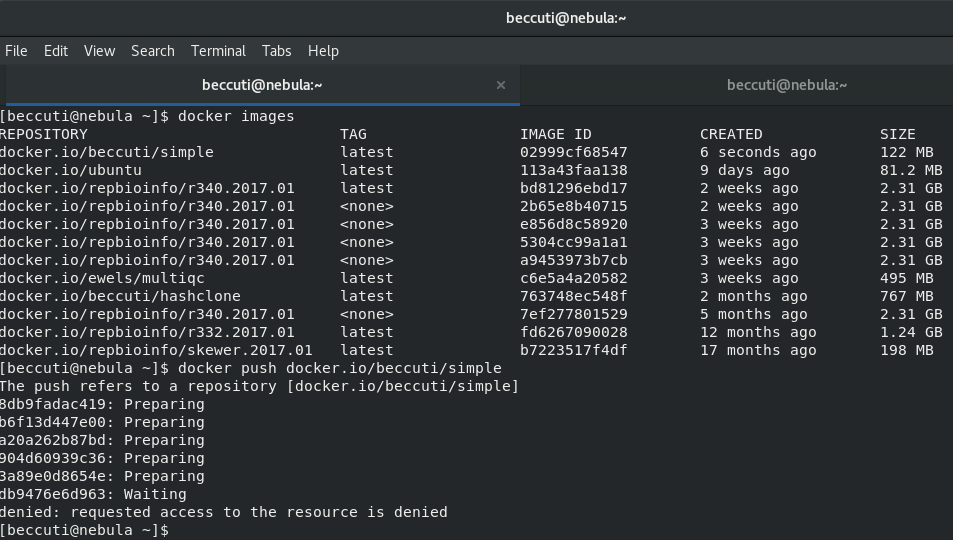
\includegraphics[width=1.00\columnwidth]{./Figure/push}
  		\end{center}  
  
  \vspace{0.2cm}
 \centerline{\textbf{\color{NavyBlue}User  must be logged into the repository}}	
 }	
 
        \frame{
\frametitle{Building a Docker Image} 
  
 \emph{\color{PineGreen} docker login}  can be exploited to login into the repository.
     	\begin{center}
  			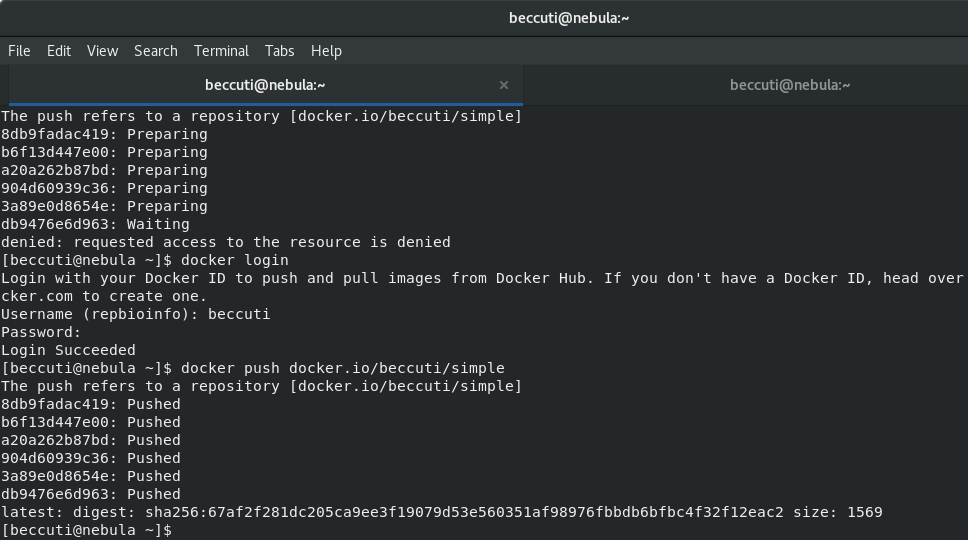
\includegraphics[width=1.00\columnwidth]{./Figure/login1}
  		\end{center}  
 }	
  	
  	
  	      \frame{
\frametitle{Building a Docker Image} 
  
 \emph{\color{PineGreen} docker push 
 $\langle \it{image} \rangle$} can be used to upload a docker image into  a hub.
     	\begin{center}
  			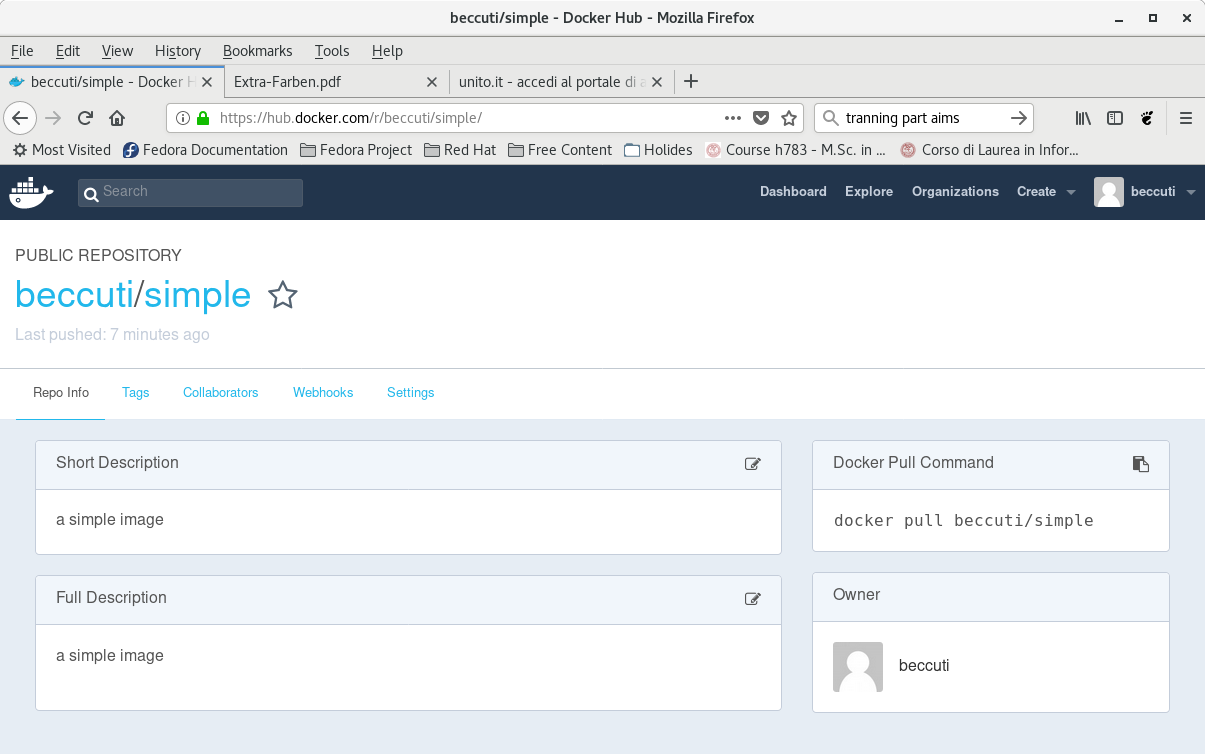
\includegraphics[width=0.90\columnwidth]{./Figure/push2}
  		\end{center}  
  
 } 	
  		 
  		 
  		 
        \frame{
\frametitle{Building a Docker Image with R} 

Install R environment in the docker image previously created.
 		     	\begin{center}
  			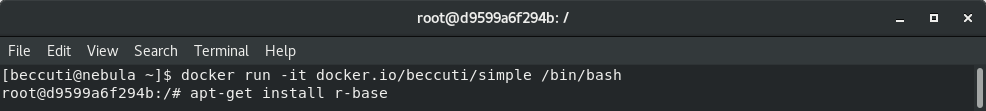
\includegraphics[width=1.00\columnwidth]{./Figure/installR}
  		\end{center}  
\vspace{0.2cm} Update our docker image.
  		
 		     	\begin{center}
  			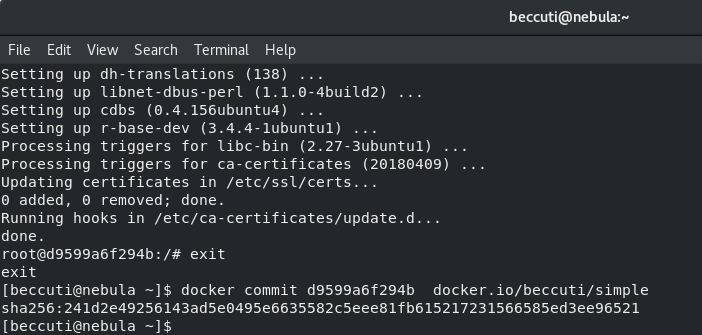
\includegraphics[width=1.00\columnwidth]{./Figure/commit3}
  		\end{center}    		
 } 	  		 
  
 
 
  		 
        \frame{
\frametitle{Building a Docker Image with R} 

A Docker image with R base is already available 
 		     	\begin{center}
  			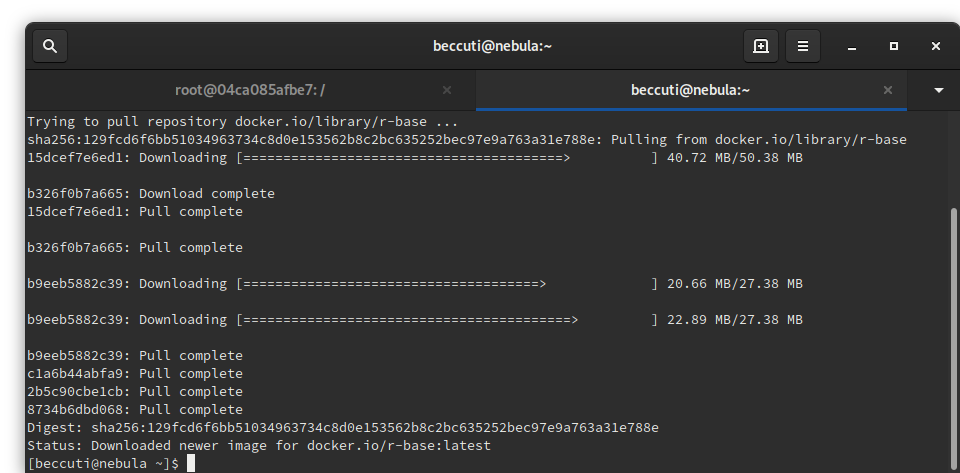
\includegraphics[width=1.00\columnwidth]{./Figure/installRbase}
  		\end{center} 
 }
 
 
         \frame{
\frametitle{Building a Docker Image with R} 

Comparing image dimensions:
 		     	\begin{center}
  			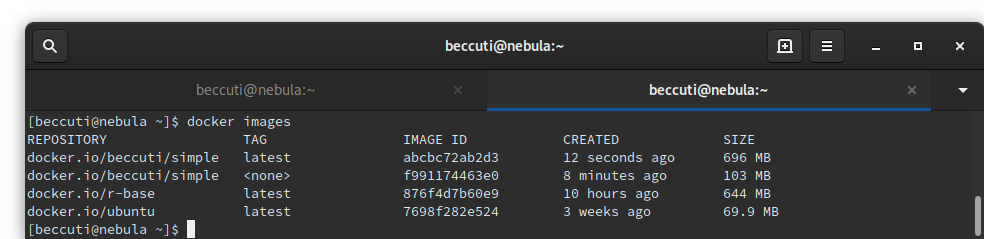
\includegraphics[width=1.00\columnwidth]{./Figure/installRbase2}
  		\end{center} 
 }
  
  
    \frame{
  \frametitle {Our first simple Docker image}
 To create this image we will perform the following tasks:\vspace{0.4cm}
 \begin{itemize}
 \item Create an own docker public repository;\vspace{0.2cm}
 \item Download a  base image from the Docker Hub;\vspace{0.2cm}	
 \item Updating the download image and upload it on our own repository;\vspace{0.2cm}	
 \item Create and embed  simple BASH and R  scripts on our image;\vspace{0.2cm}	
 \item Execute the new created image.
 \end{itemize}
} 
   
  
         \frame{
\frametitle{Our first simple Docker image} 

\textbf{\color{NavyBlue}Create R and Bash scripts.}
\begin{itemize}
\item We use \textbf{\color{NavyBlue}Rstudio} to create our  R script; %\vspace{-0.1cm}
 \begin{center}
  			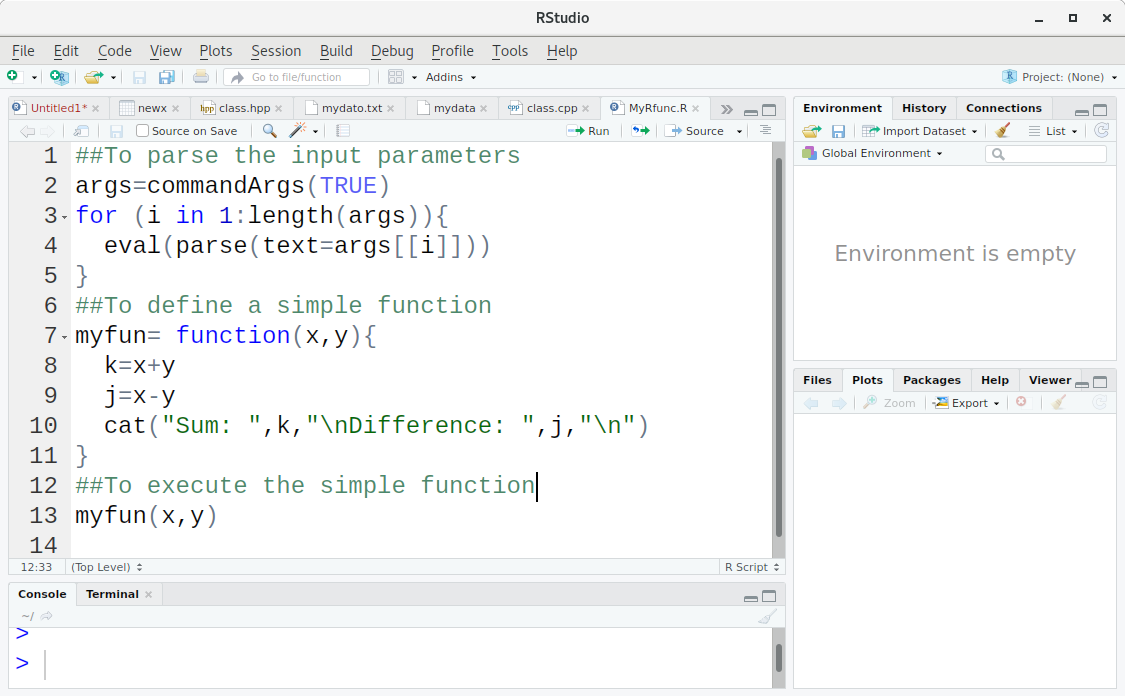
\includegraphics[width=0.93\columnwidth]{./Figure/rscript}
 \end{center} \vspace{-0.1cm}
It takes as input two vectors x and y returns their sum and difference. 
 \end{itemize}
 } 	  		 
  	
  		 
\frame{
\frametitle{Our first simple Docker image} 

\textbf{\color{NavyBlue}Create R and Bash scripts.}\vspace{0.1cm}
\begin{itemize}
\item We use \textbf{\color{NavyBlue}gedit} to create our Bash script; \vspace{0.2cm}
 \begin{center}
  			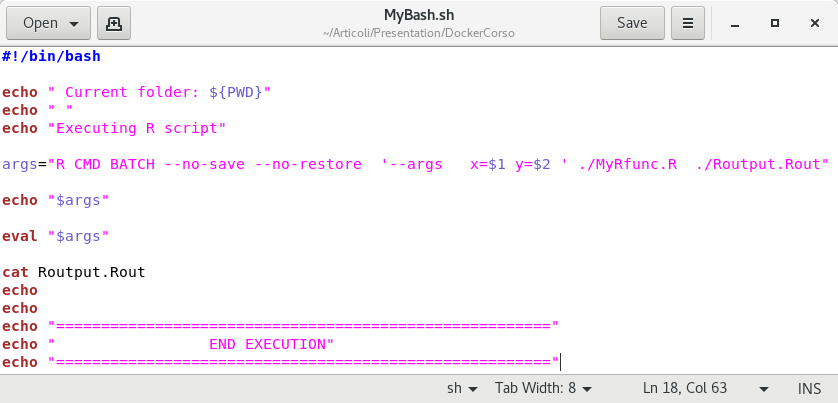
\includegraphics[width=0.93\columnwidth]{./Figure/shscript}
 \end{center} \vspace{0.2cm}
 It takes as input the two values and calls the R script previously created. 
 \end{itemize}
 } 	
 

   	  
         \frame{
\frametitle{Our first simple Docker image} \vspace{0.3cm}
Copy the two scripts in the docker image \vspace{0.2cm}
 		     	\begin{center}
  			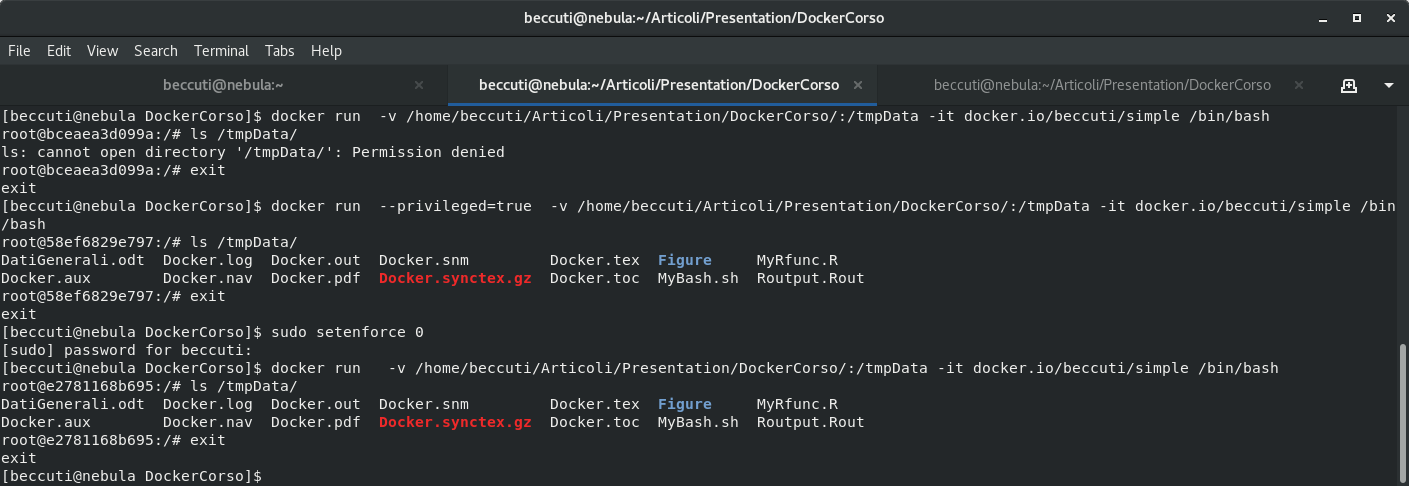
\includegraphics[width=1.00\columnwidth]{./Figure/run3}
  		\end{center}  	
 	   	  
\begin{itemize}
\item  Option \emph{\color{PineGreen}-v} is used to mount a local folder  as a volume into the container;\vspace{0.2cm}
\item If you cannot access the volume in the container then the security level  of your machine could be too stringent;\vspace{0.2cm}
\item Option  \emph{\color{PineGreen} -\;-privileged=true} can be exploited to cope with this.
\end{itemize}
   

}	  
  
       \frame{
\frametitle{Our first simple Docker image} \vspace{0.3cm}
Copy the two scripts in the docker image \vspace{0.2cm}
 		     	\begin{center}
  			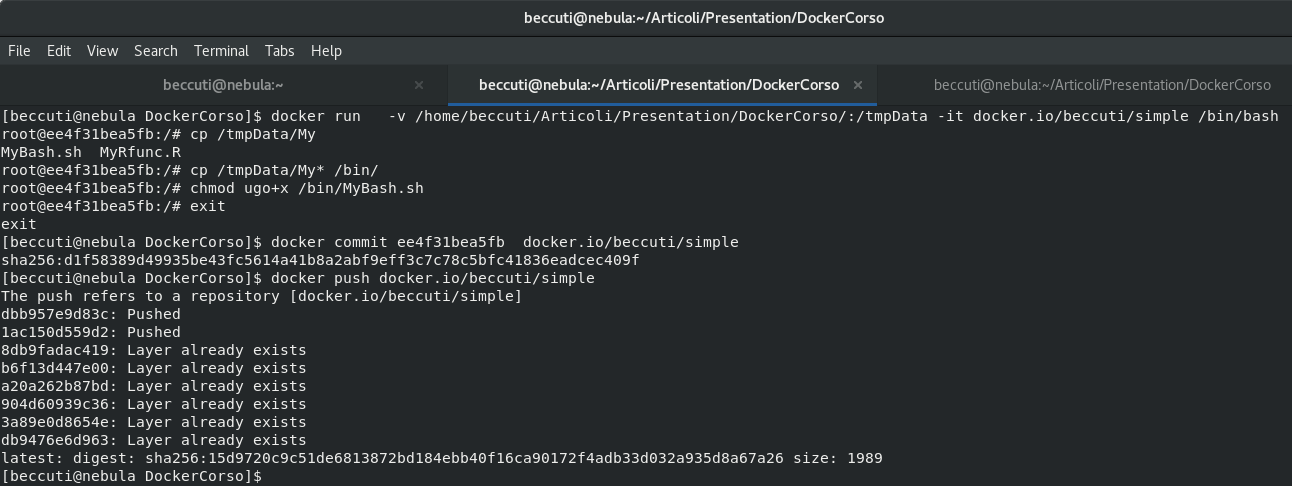
\includegraphics[width=1.00\columnwidth]{./Figure/run5}
  		\end{center}  	
  		}
  
  
  

 	
 	
 	          \frame{
\frametitle{Our first simple Docker image} 
To execute the script passing two input parameters
 		     	\begin{center}
  			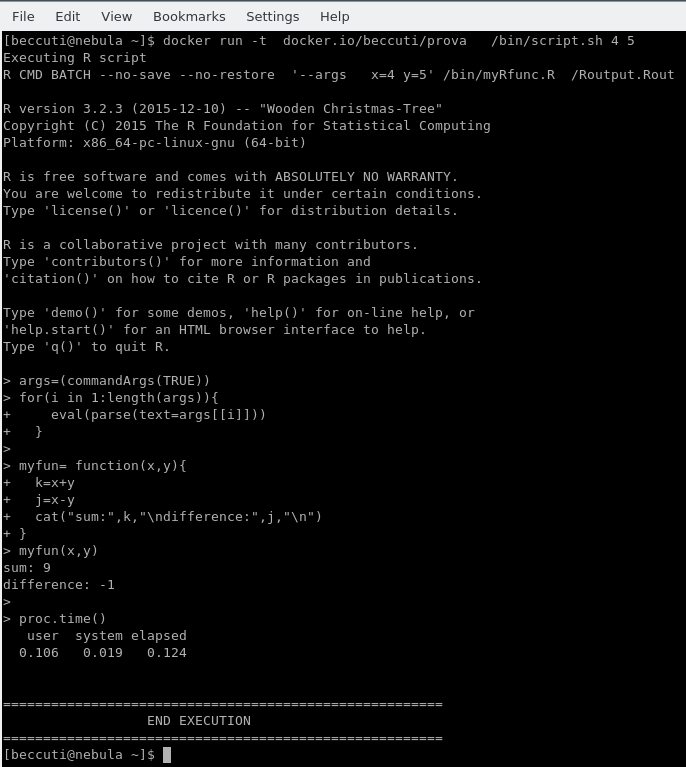
\includegraphics[width=0.80\columnwidth]{./Figure/run4}
  		\end{center}  	
 } 	
 
 
 
  \frame{
\frametitle{Our first simple Docker image} 
\begin{columns}[T] % align columns
  \begin{column}{.26\textwidth}
  \vspace{4cm}
   \hspace{0.25cm}Expected output of\\ 
     \hspace{0.25cm}our script: 
   \end{column}%
   \hfill%
   \begin{column}{0.85\textwidth}
   \vspace{-0.3cm}
    \begin{center}
  			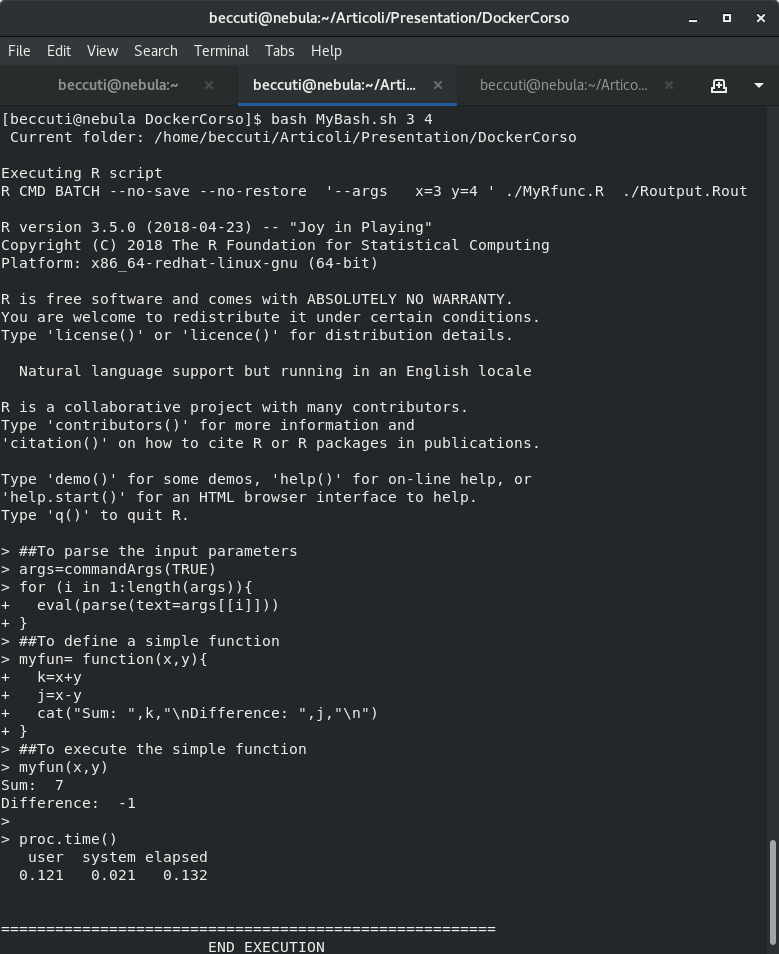
\includegraphics[width=0.70\columnwidth]{./Figure/shscript1}
 \end{center}
      \end{column}%
   \end{columns}

 } 	
   	  